%%
%    * ----------------------------------------------------------------
%    * "THE BEER-WARE LICENSE" (Revision 42/023):
%    * Ronny Bergmann <mail@rbergmann.info> wrote this file. As long as
%    * you retain this notice you can do whatever you want with this
%    * stuff. If we meet some day and you think this stuff is worth it,
%    * you can buy me a beer or a coffee in return.
%    * ----------------------------------------------------------------
%
%
% A german example using the Kartei.cls - including print and toc as
% options, hence all pages are Din A4.
%
% Last Change: Kartei 1.9, 2012/01/04
%
\documentclass[a6paper,10pt,grid=front%
,toc
%,print
]{kartei}
\usepackage[utf8]{inputenc} %UTF8
\usepackage{hyperref}
\begin{document}
  \setcardpagelayout

  \section*{ANS08}

  \begin{karte}{Definition Data Warehouse}    
    Ein Data Warehouse dient dazu, Daten aus unterschiedlichen internen und externen Quellen zusammenzuführen und zu speichern, um anschließend mithilfe unterschiedlicher Abfrage-, Analyse- und Auswertungsprogrammen neue Informationen zu gewinnen.
  \end{karte}

  \begin{karte}{Worin besteht der Unterschied zwischen operativen \& analytischen Daten?}
    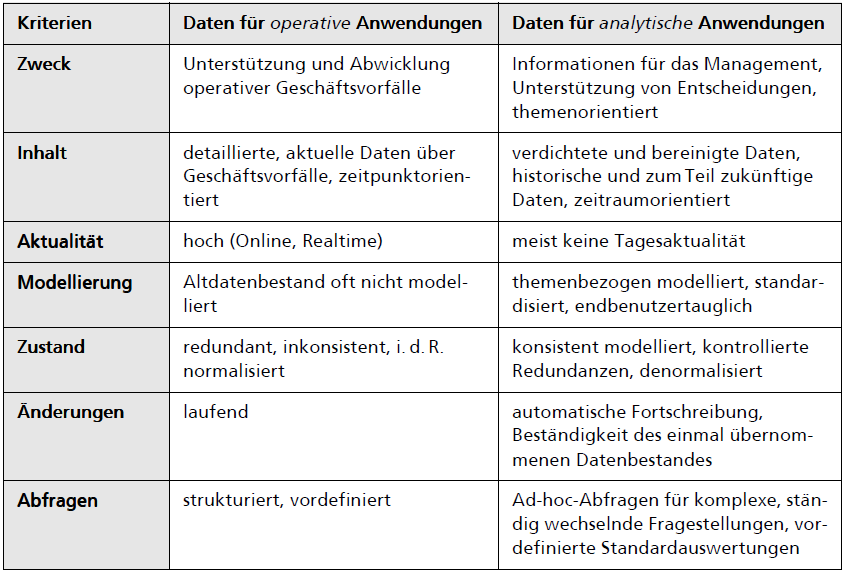
\includegraphics[width=0.9\textwidth]{img/diff_operativ_analytische_daten}
  \end{karte}

  \begin{karte}{Ziele eines Data Warehouse?}
    \begin{itemize}
      \item Informationen für das Management
      \item Unterstützung von Entscheidungen
      \item zusammenführen unterschiedlicher Daten aus operativen Anwendungssystemen
      \item es werden (un-)strukturierte Daten übernommen
      \item Veränderung, Aggregation der Daten
    \end{itemize}
  \end{karte}

  \begin{karte}{Aufbau analytischer Informationssysteme}
    \begin{itemize}
      \item \textbf{Zentrales DWH} enthält eine von den operativen Systemen isolierte Datenbank
      \item \textbf{Data Mart} ist ein subjektspezifisches oder abteilungsspezifisches DWH; entweder Datenbestände gleichzeitig an mehreren Orten schneller bereitzustellen oder einzelne Fachabteilungen spezifische Daten zu liefern
    \end{itemize}
    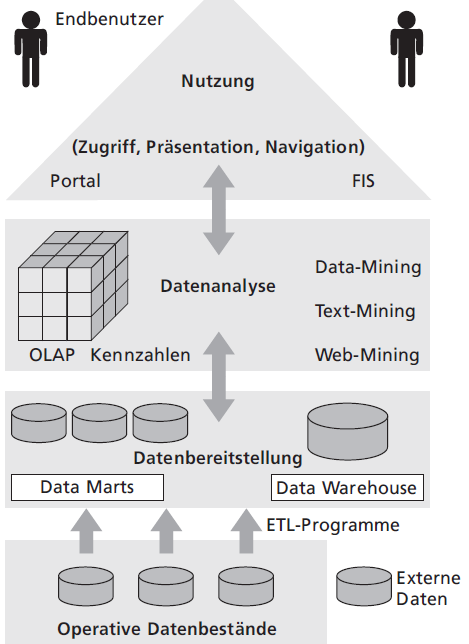
\includegraphics[height=0.5\paperheight]{img/aufbau_analytischer_is}    
  \end{karte}

  \begin{karte}{Unterschied Data Warehouse \& Data Mart}
    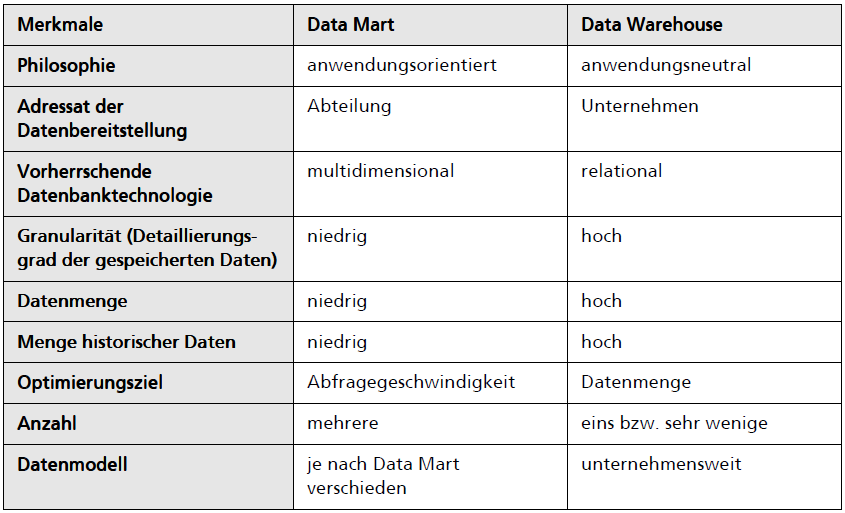
\includegraphics[width=0.9\paperheight]{img/diff_dwh_dm}
  \end{karte}

  \begin{karte}{Ablauf ETL?}
    \begin{itemize}
      \item Analyse und Dokumentation operativer und externer Datenquellen
      \item Extrahieren der ausgewählten Daten
      \item Transformation operativer Daten
      \item Bereinigung transformierter Daten
      \item periodisches Laden der Daten ins DWH
    \end{itemize}
  \end{karte}

  \begin{karte}{Extraktion}
    Unter Extraktion versteht man die Selektion der Daten aus den (zumeist) operativen Datenquellen und ihre anschließende Speicherung in einen Arbeitsbereich des DWH (Staging Area). Hier werden die Daten zwischengespeichert und transformiert bzw. bereinigt und im Anschluss in das DWH übertragen.
  \end{karte}

  \begin{karte}{Wann wird die Extraktion durchgeführt?}
      \begin{itemize} 
      \item Periodisch
      \item Anfrage
      \item Ereignisgesteuert (wenn z.B. Werte unterschritten werden)
      \item Sofort (DWH hat die gleiche Aktualität wie die operativen Systeme)
    \end{itemize}
  \end{karte}

  \begin{karte}{Transformation}
      Transformation findet in der s.g. Staging Area statt und bereinigt bzw. transformiert die Quelldaten in das gewünschte Zielformat.
  \end{karte}

  \begin{karte}{Qualitätsmängel der Quelldaten}
    \begin{itemize} 
      \item inkorrekte Daten (Eingabe-/Verarbeitungsfehler)
      \item logisch widersprüchliche Daten
      \item unvollständige, ungenaue, zu grobe Daten
      \item redundante Daten
      \item uneinheitliche Daten
      \item veraltete Daten
      \item irrelevante Daten
      \item unverständliche Daten (wegen qualitativ mangelhafter Metadaten)
    \end{itemize}

    \textbf{Verfahren:}
    \begin{itemize}
      \item Bereinigung
      \item Harmonisierung (betriebswirtschaftlich: Codierung, Schlüssel, Attribute)
      \item Verdichtung (für Analysezwecke aggregiert werden $\rightarrow$ Regionalzahlen usw.)
      \item Anreicherung (Ergänzung um errechnete Kennzahlen)
    \end{itemize}
  \end{karte}

  \begin{karte}{Bereinigung - Was ist zu beachten?}
    \begin{itemize} 
      \item Muss-Feld?
      \item Plausibilitätsprüfung bei der Eingabe?
      \item Wir das Feld gemäß der ursprünglichen Bestimmung genutzt?
      \item Wurde das Datenfeld nachträglich aufgenommen? (fehlt bei älteren Daten dann)
      \item Existieren konkrete Änderungspläne für die operativen Daten?
    \end{itemize}    
  \end{karte}

  \begin{karte}{Daten-Mängel}
    Es werden \textbf{syntaktische} und \textbf{semantische} Mängel unterschieden.

    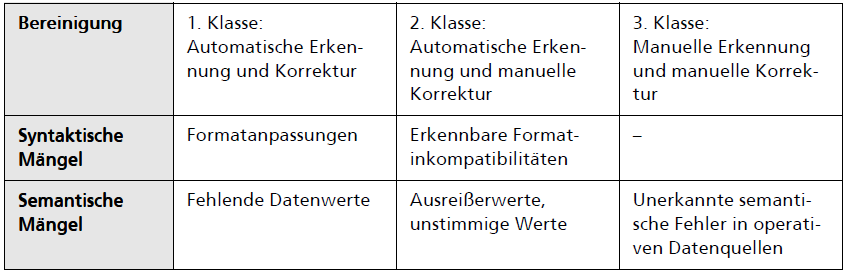
\includegraphics[width=0.9\textwidth]{img/maengel}
  \end{karte}

  \begin{karte}{Harmonisierung - Was wird getan?}
    \begin{itemize}
      \item Vereinheitlichung unterschiedlicher Codierungen (z.B. männlich, m, 1, weiblich, w, 0)
      \item Synonyme und Homonymen (unterschiedliche Attributnamen mit gleicher Bedeutung z.B. vorname, vname, firstname)
      \item Harmonisierung von Schlüsseln und Kennzahlen      
    \end{itemize}
  \end{karte}

  \begin{karte}{Verdichtung}
    Es werden Daten im DWH (Staging Area) auf verschiedenen Stufen aufsummiert.
    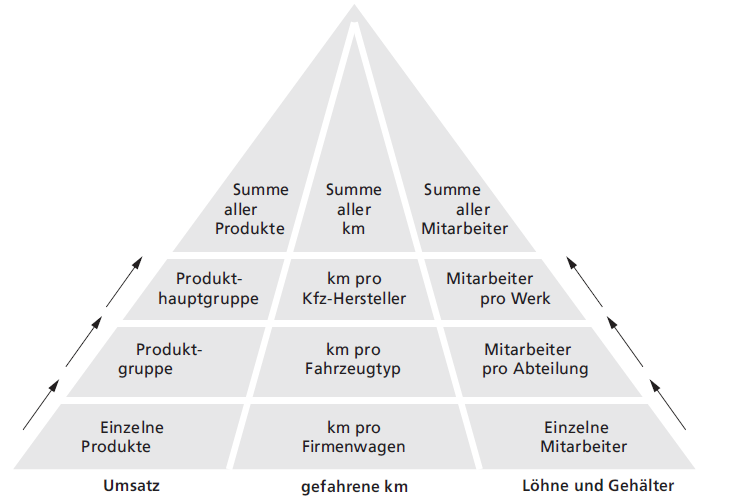
\includegraphics[width=0.9\textwidth]{img/verdichtung}
  \end{karte}

  \begin{karte}{Anreicherung}
    Es werden Berechnungen durchgeführt, die zusammen mit den übrigen analytischen Daten gespeichert werden, d.h. es werden konkrete Kennzahlen ermittelt basierend auf einem gegeben Kennzahlensystem (z.B. DuPont-Schema $\rightarrow$ ROI)

    Vorteile der Anreicherung sind:
    \begin{itemize}
      \item kürzere Antwortzeiten bei späteren Anfragen da es sich um vorberechnete Werte handelt
      \item hohe Datenkonsistenz, da sie nach einem einheitlichen Algorithmus berechnet werden
    \end{itemize}
  \end{karte}  

  \begin{karte}{Laden}
    Es wird unterschieden zwischen:
    \begin{itemize}  
      \item Initialem Füllen aus den operativen Datenbanken
      \item Zyklischer Aktualisierung, neue Werte werden ergänzt, alte archiviert
    \end{itemize}

    Wenn die Daten zyklisch übernommen werden kann dies als:

    \begin{itemize}
      \item Kompletter Abzug (einfach aber zeitaufwendig)
      \item jeweilige Änderungen (geringe Datenmenge, aufwendig das Delta zu ermitteln, nur der letzte Stand wird ermittelt)
      \item Auswahl protokollierter Datenbanktransaktionen (auch Änderungen innerhalb des Deltas erfasst werden)
    \end{itemize}

    geschehen.
  \end{karte}

  \begin{karte}{Metadaten}
    Metadaten sind Daten über Daten und enthalten Hintergrundinformationen über die im DWH gespeicherten Werte. Sie geben Aufschluss über:
    \begin{itemize}
      \item Umfang der verfügbaren Daten
      \item Datenstruktur und Beziehungen (Relationen)
      \item Herkunft der operativen Daten
      \item Speicherort im DWH
      \item Formate
      \item Zugriffsberechtigungen      
    \end{itemize}

    In der Metadatenbank wird festgehalten:

    \begin{itemize}
      \item Welche Daten woher kommen
      \item Wie sie aufbereitet und verdichtet werden
      \item Wo sie gespeichert werden
      \item Welcher Anwender auf welche Daten Zugriff erhält
    \end{itemize}
  \end{karte}

  \begin{karte}{Archivierung}  
    Es wird zwischen der:

    \begin{itemize}
      \item Datenarchivierung (auslagern auf Offlinedatenträger nach Zeit)
      \item Datensicherung (Dienen zur Wiederherstellung des DWH)
    \end{itemize}

    unterschieden.
  \end{karte}

  \begin{karte}{OLAP}  
    Der Begriff steht für Online Analytical Processing und umfasst alle Formen der \textit{mehrdimensionalen Datenanalyse}. Im Focus stehen betriebswirtschaftliche Kennzahlen. Die Mehrdimensionalität wir durch s.g. \textit{Datenwürfel} veranschaulicht.

    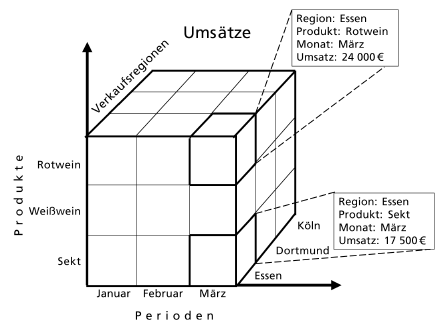
\includegraphics[height=0.65\paperheight]{img/wuerfel}
  \end{karte}

  \begin{karte}{Unterschied OLAP/TLTP}  
    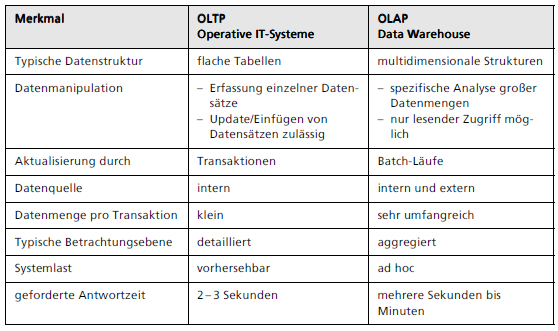
\includegraphics[width=0.9\textwidthg]{img/diff_olap_oltp}
  \end{karte}

  \begin{karte}{Anforderungen an OLAP}  
        
    \begin{itemize}
      \item Mehrdimensionale konzeptionelle Sicht auf die Daten (Zeit, Produktgruppe, Region, Person, usw.)
      \item Transparenz (Anwender müssen keine technischen Details kennen)
      \item Zugriffsmöglichkeiten (auf möglichst viele heterogene und interne/externe Datenquellen)
      \item Stabile Antwortzeiten (möglichst schnell und vor allem gleichbleibend)
      \item Client-/Server-Architektur
      \item Gleichrangige Dimensionen
      \item Dynamische Handhabung \"dünn besetzter\" Matrizen (effiziente Speicherung trotz Lücken)
      \item Mehrbenutzerfähigkeit
      \item Unbeschränkt dimensionsübergreifende Operationen
      \item Intuitive Datenanalyse
      \item Flexibles Berichtswesen (Dokumentation in FOrm von Berichten und Grafiken)
      \item Unbegrenzte Anzahl von Dimensionen/Aggregationsstufen
    \end{itemize}

    \textbf{Kritik:} Die unscharfe Trennung zwischen fachlich-konzeptionellen Anforderungen und technischer Realisierung.

    Alternativ \textbf{FASMI}:

    \begin{itemize}
      \item Fast (Antwortzeit max. 20s)
      \item Analysis (Anwender ohne technisches Wissen müssen auswerten können)
      \item Shared (Mehrbenutzer)
      \item Multidimensional
      \item Information (sämtliche benötigten Informationen können geliefert werden)      
    \end{itemize}
  \end{karte}

  \begin{karte}{Mehrdimensionalität}  
    Die Anzahl der Dimensionen lässt sich mit der Fakultät der Dimensionen berechnen:
    2 Dim = 1 x 2 = 2 Sichten\\
    3 Dim = 1 x 2 x 3 = 6 Sichten\\
    4 Dim = 1 x 2 x 3 x 4 = 24 Sichten\\

    Die verschiedenen Betrachtungsmöglichkeiten werden auch als \textbf{Slice and Dice} bezeichnet. \textit{Slice} bedeutet das Herausschneiden von Scheiben aus dem Würfel. \textit{Dice} bedeutet die Bildung von kleinen Würfeln aus dem Gesamtwürfel zur Einschränkung auf einen Wert bzw. Wertebereich.

    Mittels \textbf{Drill down} ist es möglich von einer bestehenden Verdichtungsebene auf eine detaillierte Ebene zu wechseln. \textbf{Drill up} wechselt von einer Ebene auf eine verdichtertere Ebene. \textbf{Drill across} ermöglicht zu einem anderen Wert auf der selben Ebene zu wechseln.
  \end{karte}

  \begin{karte}{Wie können Daten verdichtet werden?}  
    
    Wie die Daten verdichtet werden können hängt unmittelbar vom Typ ab.

    \begin{itemize}
      \item \textbf{Additive Daten} lassen sich beliebig aufsummieren (Umsatz in Kombination mit Produkten und Regionen)
      \item \textbf{Semiadditive Daten} lassen sich nicht über alle Dimensionen aufaddieren (z.B. bei Zeiträumen und Lagerbeständen)
      \item \textbf{Nichtadditive Daten} lassten keine sinnvolle Aufsummierung zu (Anteilswerte)
    \end{itemize}
  \end{karte}

  \begin{karte}{Modellierung}    
    Die \textbf{multidimensionale Modellierung} ist in der Lage die konzeptionellen Datenstrukturen in physische Datenbank-/Speicherstrukturen umzusetzen. Im Falle eine \textit{dünn besetzen Matrix} wird Speicherplatz vergeudet, da für nicht existente Werte gleich viel Speicher verbraucht wird, als wenn der Wert existiert.

    Die \textbf{relationale Modellierung} setzt die mehrdimensionale Datenstruktur in einer relationalen Datenbankstruktur ab. Es wird dabei zwischen:

    \begin{itemize}
      \item Fakten (quantitative Kerndaten)
      \item Dimension (beschreibende Daten, kann beliebig viele Ausprägungen haben)
    \end{itemize}

    unterschieden.
  \end{karte}

  \begin{karte}{Star-Schema}  
    Für jede Dimension wird eine Tabelle eingerichtet. Die Dimensionstabellen sind nicht miteinander verknüpft, sondern stehen nur über die Faktentabelle miteinander in Beziehung. Der Primärschlüssel in der Faktentabelle setzt sich zusammen aus den Primärschlüsseln aller Dimensionstabellen.

    Vorteil:
    \begin{itemize}
      \item einfaches, intuitive Datenmodell
      \item benötigt nur wenige Join-Operationen
      \item wenige Tabellen benötigt
    \end{itemize}

    Nachteil:
    \begin{itemize}
      \item durch die große Anzahl der Verknüpfungsmöglichkeiten
kann es zu Performanceproblemen kommen
    \end{itemize}
    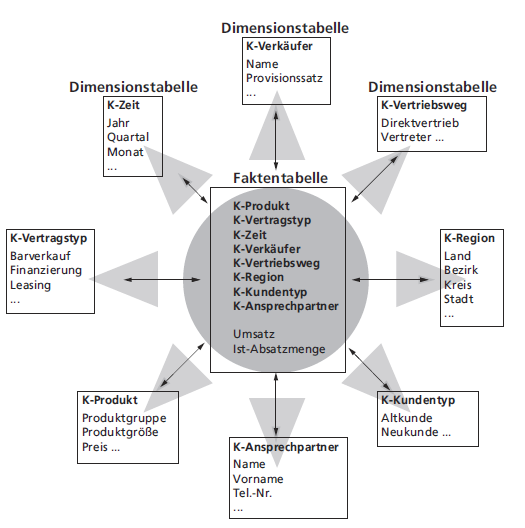
\includegraphics[height=0.45\paperheight]{img/star_schema}
  \end{karte}

  \begin{karte}{Snowflake-Schema}  
    Dieses Schema ist einer Erweiterung des Star-Schemas und wird durch die Normalisierung entwickelt.

    Vorteile:
    \begin{itemize}
      \item erleichtert die Aggregation
      \item keine Redundanzen      
    \end{itemize}

    Nachteile

    \begin{itemize}
      \item höhere Anzahl JOINS
      \item höhere Anzahl Tabellen
      \item komplexere SQL-Abfragen
    \end{itemize}

    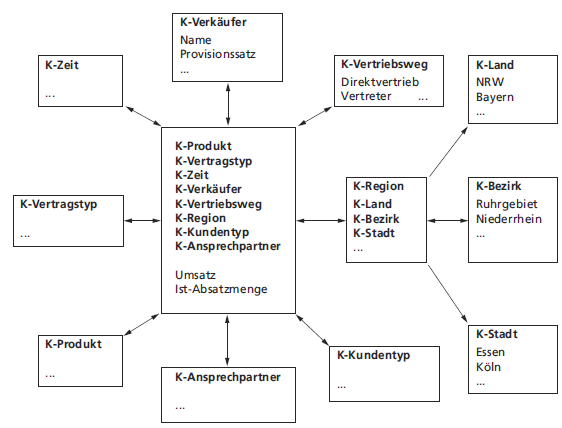
\includegraphics[height=.45\paperheight]{img/snowflake}
  \end{karte}

  \begin{karte}{Was ist Data-Mining?}
    
  \end{karte}
\end{document}